\documentclass[times, utf8, zavrsni]{fer}
\usepackage{booktabs}
\usepackage{listingsutf8}
\usepackage{float}
\usepackage[T1]{fontenc}
\usepackage[scaled]{beramono}
\usepackage{xcolor}
\usepackage{caption}

\definecolor{bluekeywords}{rgb}{0,0,1}
\definecolor{greencomments}{rgb}{0,0.5,0}
\definecolor{redstrings}{rgb}{0.64,0.08,0.08}
\definecolor{xmlcomments}{rgb}{0.5,0.5,0.5}
\definecolor{types}{rgb}{0.17,0.57,0.68}

\usepackage{listings}
\lstdefinestyle{csharp}
{
language=[Sharp]C,
captionpos=b,
showspaces=false,
showtabs=false,
breaklines=true,
showstringspaces=false,
breakatwhitespace=true,
escapeinside={(*@}{@*)},
commentstyle=\color{greencomments},
morekeywords={partial, var, value, get, set},
keywordstyle=\color{bluekeywords},
stringstyle=\color{redstrings},
basicstyle=\fontsize{10}{10}\selectfont\ttfamily,
aboveskip=1em,
belowskip=0.75em
}

\lstdefinestyle{sql}
{
language=SQL,
showspaces=false,
showtabs=false,
tabsize=4,
breaklines=true,
showstringspaces=false,
breakatwhitespace=true,
escapeinside={(*@}{@*)},
commentstyle=\color{greencomments},
keywordstyle=\color{bluekeywords}\bfseries,
stringstyle=\color{redstrings},
inputencoding=utf8/latin2,
basicstyle=\fontsize{10}{10}\selectfont\ttfamily,
frame=single,
aboveskip=1em,
belowskip=0.75em
}

\lstdefinestyle{html}
{
language=html,
showspaces=false,
showtabs=false,
tabsize=4,
breaklines=true,
showstringspaces=false,
breakatwhitespace=true,
escapeinside={(*@}{@*)},
commentstyle=\color{greencomments},
keywordstyle=\color{bluekeywords}\bfseries,
stringstyle=\color{redstrings},
inputencoding=utf8/latin2,
basicstyle=\fontsize{10}{10}\selectfont\ttfamily,
frame=single,
aboveskip=1em,
belowskip=0.75em
}

\lstdefinelanguage{JavaScript}{
keywords={typeof, new, true, false, catch, function, return, null, catch, switch, var, if, in, while, do, else, case, break},
keywordstyle=\color{blue}\bfseries,
ndkeywords={class, export, boolean, throw, implements, import, this},
ndkeywordstyle=\color{darkgray}\bfseries,
identifierstyle=\color{black},
sensitive=false,
comment=[l]{//},
morecomment=[s]{/*}{*/},
commentstyle=\color{purple}\ttfamily,
stringstyle=\color{red}\ttfamily,
morestring=[b]',
morestring=[b]"
}

\lstdefinestyle{js}
{
language=JavaScript,
showspaces=false,
showtabs=false,
tabsize=4,
breaklines=true,
showstringspaces=false,
breakatwhitespace=true,
escapeinside={(*@}{@*)},
commentstyle=\color{greencomments},
keywordstyle=\color{bluekeywords}\bfseries,
stringstyle=\color{redstrings},
inputencoding=utf8/latin2,
basicstyle=\fontsize{10}{10}\selectfont\ttfamily,
frame=single,
aboveskip=1em,
belowskip=0.75em
}

\begin{document}

\thesisnumber{4439}

\title{Baza podataka i Web aplikacija za upravljanje vremenom tijekom studija}

\author{Vedran Biđin}

\maketitle
\begin{figure}[H]
\centering

\includegraphics[width=\textwidth]{img/izvornik.pdf}
\label{izvornik}
\end{figure}

\zahvala{}

\tableofcontents

\chapter{Uvod}
Rad obuhvaća oblikovanje modela baze podataka za praćenje vremena utrošenog na aktivnosti tijekom studija, te izradu pripadne web aplikacije za navedenu bazu podataka, koja omogućuje korisnicima, odnosno studentima, da evidentiraju i pregledavaju svoje utrošeno vrijeme preko odgovarajućih korisničkih sučelja web aplikacije.

Baza podataka opisana je u cijelosti u 2. poglavlju rada, počevši sa opisom zahtjeva baze gdje se definiraju zahtjevi korisnika, kao i odgovarajući podaci i njihova struktura koje je potrebno pohraniti u bazi podataka. Nakon toga slijedi definicija konceptualnog ER modela baze zajedno sa pripadajućim objašnjenjima i dijagramom, te napokon relacijski model baze koji predstavlja stvarnu, fizičku bazu podataka kakvu je koristi web aplikacija tijekom rada.

Web aplikacija opisana je u 3. poglavlju. Prvo se spominju tehnologije i alati koji su korišteni tijekom njene izrade, nakon čega se opisuje sama implementacija. Web aplikacija je podijeljena na 4 dijela, svaki od kojih opisuje jednu samostalnu cjelinu web aplikacije koja se sastoji od pripadajućeg korisničkog sučelja, podataka, i poslovne logike. Kroz opise cjelina spominju se i određene tehnologije koje omogućuju dodatne funkcionalnosti a koje su specifične za svaku cjelinu web aplikacije. Nakon opisa web aplikacije dodatno se spominju načini kojima bi se baza podataka i web aplikacija mogli unaprijediti i nadograditi.

\chapter{Baza podataka}

\section{Opis problema}
Web aplikacija mora omogućiti korisnicima, odnosno studentima, da evidentiraju vrijeme koje su utrošili tijekom studija na aktivnosti kao što su direktna nastava, učenje, te ostale nastavne obaveze studenata. Sustav također mora omogućiti korisnicima da pregledavaju utrošeno vrijeme te da uspoređuju stvarno utrošeno vrijeme sa vremenom koje je ECTS bodovima propisano za uspješno svladavanje nastavnih obaveza.

Zadatak stvaranja baze podataka web aplikacije podrazumijeva dizajn sheme baze. Potrebe korisnika igraju središnju ulogu u konstruiranju sheme. Početna faza dizajna baze podrazumijeva opisivanje potrebe potencijalnih korisnika. Ishod ove faze u složenijim aplikacijama mogla bi biti specifikacija zahtjeva korisnika. Nakon što su definirani svi zahtjevi, iz njih se izvodi konceptualni model baze podataka.
\begin{enumerate}[leftmargin=*]
\item Svaki korisnik mora moći evidentirati te pregledavati svoje utrošeno vrijeme - sustav mora moći razlikovati korisnike. To se obično postiže tako da svaki korisnik ima na raspolaganju svoj vlastiti korisnički račun, te se sve evidencije koje on provodi implicitno vežu na njegov korisnički račun. Potrebno je implementirati tipični sustav za prijavljivanje, koji omogućuje korisnicima da se prijave na svoj korisnički račun uporabom korisničkog imena i lozinke, ili da naprave novi račun sa svim potrebnim podacima u slučaju ako nemaju već postojeći korisnički račun. Također je korisnicima potrebno omogućiti neke osnovne funkcionalnosti poput mijenjanje postojećih korisničkih podataka kao što su lozinka, e-mail, i slično.

\item Korisnik mora moći evidentirati svoje utrošeno vrijeme. Evidencija vremena međutim mora biti na neki način vezana uz određenu aktivnost ili nastavnu obavezu. Nema smisla da korisnik samo evidentira utrošeno vrijeme, jer to može značiti da je vrijeme utrošeno na apsolutno bilo koji dio studija, a takve evidencije ne pružaju ikakvu informaciju vrijednu sakupljanja niti pregleda. Dakle, korisnik mora moći na neki (intuitivni) način u sustavu pronaći svoju specifičnu aktivnost.

\item Korisniku je potrebno omogućiti pregled svog trenutačnog utrošenog vremena, i to na taj način tako da se može uspoređivati stvarno utrošeno vrijeme korisnika sa vremenom koje je propisano ECTS bodovima, semestralnim opterećenjima, ili na bilo koji drugi način. Da bi to bilo moguće, potrebno je aktivnosti koje korisnik može evidentirati podijeliti na neki način u grupe i propisati im određene očekivane iznose utrošenog vremena koje bi one trebale iznositi. Korisnik bi trebao moći vidjeti ne samo koliko je vremena on utrošio na neku aktivnost i koliko je vremena 'trebao' utrošiti, nego i koliko je vremena utrošio na sve 'pod-aktivnosti' te aktivnosti (pošto neke aktivnosti implicitno obuhvaćaju druge aktivnosti).
\end{enumerate}

Web aplikacija podrazumijeva korištenje baze podataka. U ovom specifičnom slučaju, očito je da je baza podataka ključan dio cijelog sustava: sve aktivnosti moraju se negdje nalaziti, a iznosi utrošenog vremena moraju negdje biti pohranjeni. Potrebno je modelirati bazu tako da omogućava podjelu i grupaciju aktivnosti i pod-aktivnosti na način koji omogućava korisnicima jednostavno korištenje web aplikacije, kao i prikaz korisnih informacija tijekom pregleda utrošenog vremena.

Shema razvijena u ovoj konceptualnoj-fazi projektiranja omogućava detaljan pregled sustava. Model entitet-veza \engl{entity-relationship} obično se koristi za zastupanje konceptualnog dizajna. U takvom modelu konceptualna shema određuje objekte odnosno entitete koji su zastupljeni u bazi podataka, atribute entiteta, odnose među entitetima, te ograničenja na entitetima i vezama. Tipično, u konceptualnoj-fazi projektiranja stvara se dijagram ER modela koji pruža grafički prikaz sheme. Fokus konceptualnog ER modela je prikaz objekata i veza između njih, a ne specifičnih detalja poput načina pohrane pojedinih tipova podataka.

U izradi sheme, potrebno je osigurati da se izbjegnu dva glavna problema \citep{dbsyscon}:
\begin{enumerate}[leftmargin=*]
\item \textbf{Redundancija}: Dizajn baze podataka može duplicirati iste podatke. Primjerice, ako se uz svaku evidenciju o utrošenom vremenu zapisuje ime aktivnosti, ime aktivnosti bilo bi redundantno, pošto se naziv aktivnosti sprema za svaku spremljenu evidenciju višestruko puta, što je očito nepotrebno. Dovoljno je spremiti identifikator aktivnosti za svaku evidenciju, a ime aktivnosti spremiti zasebno u svoj vlastiti entitet, samo jednom.
\item \textbf{Nepotpunost}: Loš dizajn baze može učiniti određene dijelove problema teškim ili nemogućim za modelirati. Primjerice, ako baza sadrži samo entitet koji obuhvaća evidencije, a ne sadrži entitet za aktivnosti, onda bi bilo nemoguće prikazivati aktivnosti koje još nisu evidentirane.
\end{enumerate}

\section{ER model}
\subsection{Entiteti}
\begin{enumerate}[leftmargin=*]
\item \textbf{Korisnik} -
Kako bi korisnici bili u mogućnosti prijavljivati se na sustav sa svojim korisničkim podacima, potrebno je u bazu dodati entitet koji predstavlja korisnika i sve podatke vezane neposredno uz njega. U slučaju ove web aplikacije, nije potrebno puno komplicirati stvari - da bi se definirao korisnik potrebno je imati određeno unikatno korisničko ime po kojem se taj korisnik raspoznaje od drugih korisnika, potrebna je određena lozinka sa kojom se korisnik može prijaviti na sustav, te također e-mail adresa, koja bi omogućila korisniku vraćanje lozinke (u slučaju da je zaboravi). Pošto za ovu web aplikaciju postoji razlika između običnih korisnika i korisnika sa većim privilegijama (kao što su moderatori, odnosno administratori), potrebno je također na neki način u bazi podataka definirati koju razinu prava korisnik ima. To se može omogućiti dodavanjem atributa tipa cijelog broja koji označava privilegije korisnika (Tablica \ref{tbl:razine-prava}).

\begin{table}[H]
\caption{Razine prava korisnika}
\label{tbl:razine-prava}
\centering
\begin{tabular}{cl}
\hline
Vrijednost & Uloga\\
\hline
0 & Klijent \\
1 & Moderator \\
2 & Administrator \\ 
\hline
\end{tabular}
\end{table}

Lozinka korisnika je običan niz znakova, međutim spremiti je kao takvu u bazu podataka je loša ideja: na taj način bilo tko sa pristupom bazi podataka ima i pristup svim lozinkama korisnika te ih može zlouporabiti. Bolji način je enkriptirati lozinku te je kao takvu spremiti u bazu. Svaki puta kada se korisnik prijavljuje na sustav on unosi svoju lozinku koja se zatim ponovno enkriptira, nakon čega se enkriptirana verzija trenutno unešene lozinke uspoređuje sa onom koja se pohranila u bazu tijekom registracije tog korisnika (ili tijekom zadnje promjene lozinke). Na taj način i dalje je omogućena prijava korisnika kao i inače, ali je sama lozinka sada sigurna. Moglo bi se otići korak dalje i dodati takozvanu 'sol' \engl{salt}, da bi se daljnje povećala sigurnost lozinke, ali je to za ovakav sustav poprilično nepotrebno.\clearpage

\item \textbf{Aktivnost} - 
Potrebno je omogućiti prijavljenom korisniku da evidentira utrošeno vrijeme. Kako je ovo web aplikacija za evidenciju utrošenog vremena tijekom studija, potrebno je na neki način u bazi definirati sve aktivnosti koje je moguće evidentirati. Zato se definira entitet 'Aktivnost' koji predstavlja bilo koju aktivnost za koju se može evidentirati utrošeno vrijeme.

Svaka aktivnost ima određeno ime, primjerice: '3. laboratorijska vježba iz predmeta Mrežno Programiranje'. Aktivnost također može imati datum početka i trajanje kao što je to u slučaju laboratorijske vježbe ili određenog predavanja, te je potrebno definirati atribute 'Datum početka' i 'Trajanje'. Međutim, neke 'apstraktnije' aktivnosti ne trebaju nužno imati datum početka i trajanje - aktivnosti kao što su 'Učenje za međuispit iz predmeta Baze podataka', ili 'Izrada seminara iz predmeta Vještine komuniciranja'. U tom slučaju aktivnost neće imati datum početka, što nije problem jer se to u bazi podataka može predočiti tako da se kao vrijednost atributa zapiše NULL (Tablica \ref{tbl:tablica-trajanje}).

\begin{table}[H]
\caption{Trajanje aktivnosti}
\label{tbl:tablica-trajanje}
\centering
\begin{tabular}{lr} \hline
Aktivnost & Trajanje\\ \hline
Predavanje & 2 sata\\ 
Projekt & NULL\\
Laboratorijska vježba & \textasciitilde10 sati\\
\end{tabular}
\end{table}

Trajanje aktivnosti može se interpretirati na više načina. U slučaju neke fiksne aktivnosti kao što je to predavanje, naprimjer '5. predavanje iz predmeta Umjetna inteligencija', koje ima definiran i datum početka i trajanje, odabir trajanja je jednoznačan: trajanje samog predavanja (npr. 3 sata). U slučaju aktivnosti koje nemaju definiran početak, nema smisla ni evidentirati trajanje pa je logično da trajanje također bude NULL. Međutim za aktivnosti koje nemaju fiksno trajanje, može postojati neko 'pretpostavljeno' ili 'očekivano' vrijeme trajanja. Ako su voditelji nekog predmeta odredili da će se kao dio predmeta obrađivati seminar, očito je da je izrada seminara neko nepredviđeno vrijeme koje puno varira, ali upravo zato je zanimljivo evidentirati koliko je vremena utrošeno na seminar, te uspoređivati to vrijeme sa naprimjer prosjekom utrošenog vremena svih studenata ili nekim očekivanim vremenom koje je definirano od strane voditelja. Zato se u slučaju nepostojećeg datuma početka, trajanje definira ili kao NULL, ili kao stvarna vrijednost, u slučaju kada postoji neki očekivani vremenski period trajanja te aktivnosti.

\item \textbf{Predmet} - 
Gotovo svaka aktivnost koja se može evidentirati zapravo je vezana na neki predmet. Zato je potrebno odvojiti ime predmeta od naziva aktivnosti, te ga staviti u zasebni entitet u kojem su definirani predmeti. Zatim se definira veza između entiteta 'Aktivnost' i entiteta 'Predmet' koja definira koja aktivnost pripada sklopu kojeg predmeta. Na taj način omogućuje se korisnicima lakši odabir aktivnosti koju žele evidentirati: korisnici mogu po predmetima pretraživati aktivnosti, umjesto da su zatrpani sa tisućama mogućih aktivnosti svih predmeta, većinu od kojih ih uopće ne zanimaju. Uz to, pošto je sad svaka aktivnost vezana uz predmet, moguće je izračunati utrošeno vrijeme po svakom predmetu, umjesto samo ukupnog utrošenog vremena.

Entitet predmet, osim samog naziva predmeta, treba sadržavati i godinu održavanja predmeta, pošto je očito da se isti predmeti mogu održavati više godina zaredom, a tijekom godine mogu promijeniti svoje aktivnosti! Primjer: jedne godine predmet 'Komunikacijske mreže' obuhvaća domaće zadaće, a sljedeće godine umjesto domaćih zadaća održava se projekt, ili slično. Na ovaj način se isti predmet predavan u različitoj godini tretira kao potpuno različiti predmet, što je u ovom slučaju poželjno. Osim toga svaki predmet ima definirani iznos ECTS bodova, koji zapravo govori koliko vremena bi student trebao potrošiti na taj predmet (jedan ECTS bod je ekvivalentan ~28 sati). Važnost ECTS bodova je očito ključna, ona omogućuje usporedbu stvarnog utrošenog vremena predmeta sa očekivanim utrošenim vremenom.

Kako definirati primarne ključeve ovih entiteta? U slučaju predmeta obično postoji određena šifra koja jednoznačno definira predmet, a osim te šifre kao ključ mogao bi se koristiti kompozitni ključ 'Ime' predmeta i 'Godina', pošto ne postoji predmet koji se održava više puta iste godine (uz pretpostavku da su imena predmeta unikatna, kao što je obično istina u sklopu jednog zasebnog fakulteta, i što se uzima kao istina za ovaj završni rad). Međutim, u slučaju aktivnosti uistinu ne postoji prirodni ključ. Jedno rješenje je dodavanje novog atributa imena 'ID' koji služi kao surogatni ključ entiteta 'Aktivnost'.

Veza entiteta 'Predmet' i 'Aktivnost' je jednostavna: to je veza koja označuje koji predmet pripada kojoj aktivnosti, te nema svoje vlastite atribute nego samo sadrži primarne ključeve entiteta koje povezuje. Pošto je kardinalnost veze 1-N (1 predmet obuhvaća N aktivnosti, a svaka aktivnost pripada samo 1 predmetu), primarni ključ veze je primarni ključ entiteta na N strani veze: atribut 'ID'.\clearpage

\item \textbf{TipAktivnosti} - 
Određene aktivnosti mogu se osim po predmetu, dodatno grupirati u logičke cjeline. Aktivnosti su trenutačno grupirane po predmetima, što omogućuje pregled utrošenog vremena po predmetu, kao i po pojedinačnoj aktivnosti, međutim, određene aktivnosti predmeta međusobno su povezane ne samo po predmetima, nego i po tipovima aktivnosti. Aktivnost '1. laboratorijska vježba' i '2. laboratorijska vježba', obje iz predmeta 'Baze podataka', bi mogle oboje biti dio cjeline koja se zove 'laboratorijske vježbe'. Na ovaj način, korisnicima je još lakše evidentirati aktivnosti. Osim toga, tijekom pregleda utrošenog vremena moglo bi se uspoređivati koliko je vremena utrošeno po grupama aktivnosti, što može predstavljati jako zanimljivu informaciju. Zato se definira novi entitet imena 'TipAktivnosti', koji definira moguće tipove aktivnosti: predavanja, laboratorijske vježbe, domaće zadaće, seminare, ispite, itd.

Zatim se svaka aktivnost preko veze povezuje sa odgovarajućim tipom aktivnosti. Entitet 'TipAktivnosti' sam po sebi nije osobito zanimljiv: to je samo naziv tipa aktivnosti. Ovaj entitet sadrži relativno malen broj n-torki, broja sigurno manjeg od 100, pa nije loša ideja dodati primarni surogatni ključ 'ID', radi konzistentnosti sa ostalim dijelom baze podataka.
\end{enumerate}

\subsection{Veze}
\begin{enumerate}[leftmargin=*]
\item \textbf{Evidencija} -
Korisnicima treba omogućiti da evidentiraju svoje utrošeno vrijeme. Potrebno je definirati vezu 'Evidencija' koji predstavlja jednu evidenciju jednog korisnika za jednu aktivnost. U ovom slučaju to je veza između entiteta 'Korisnik' i 'Aktivnost', koja prikazuje koji korisnik evidentira koji predmet. Kako je kardinalnost veze N-N (jedan korisnik može evidentirati više aktivnosti, i jedna aktivnost može biti evidentirana od strane više korisnika) primarni ključ bit će unija primarnih ključeva entiteta koje povezuje: 'KorisnickoIme' i 'AktivnostID'.

Osim toga moguće je da jedan korisnik jednu aktivnost evidentira više puta, primjerice za aktivnosti poput laboratorijske vježbe moglo bi prvo biti evidentirano vrijeme utrošeno za izradu pripreme, pa zatim vrijeme na samoj laboratorijskoj vježbi, u kojem slučaju trenutačni primarni ključ ne bi bio dovoljan: više n-torki imale bi kao primarni ključ istu vrijednost, što nije dopustivo (Tablica \ref{tbl:tablica-evidencija}). 

\begin{table}[H]
\caption{Evidencije}
\label{tbl:tablica-evidencija}
\centering
\begin{tabular}{lll} \hline
Aktivnost & Trajanje & Opis\\ \hline
Završni rad & 20 sati & Izrada \emph{login} sustava\\ 
Završni rad & 15 sati & Dodano poglavlje \emph{ER model}\\
Završni rad & 7.5 sati & Promijenjen stil aplikacije\\
... & ... & ...\\
\end{tabular}
\end{table}

Zato je potrebno dodati u skup atributa primarnog ključa još jedan atribut koji razrješava prethodno navedeni slučaj. Dobar odabir bio bi 'Datum unosa', koji predstavlja datum pohranjivanja evidencije, čime se omogućuje više evidencija od strane jednog korisnika za istu aktivnost. Dalje, potrebno je definirati sam utrošak vremena, pa se dodaje vlastiti atribut veze 'Trajanje' koji predstavlja koliko vremena je utrošeno na aktivnost koju referencira evidencija. Dalje od interesa mogao bi biti eventualno opis evidencije, koji bi mogao pohranjivati dodatne informacije vezane uz evidenciju.\\

\item \textbf{Pretplata} - 
Kako bi korisnik mogao evidentirati utrošeno vrijeme za neku aktivnost, prvo mora odabrati njezin predmet, a entitet 'Predmet' može sadržavati jako velik broj predmeta. Čak i sa nekim načinom pretraživanja predmeta, korisnik bi morao tijekom svake evidencije birati 'svoj' predmet od svih mogućih (kojih može biti stotine!). Bilo bi korisno kada bi svaki korisnik mogao imati neki predefinirani skup predmeta na koje je 'pretplaćen', te da mu se tijekom evidencije i pregleda pokazuju samo ti predmeti. Zato se uvodi nova veza 'Pretplata' koja povezuje entitet 'Korisnik' i 'Predmet', čime se može u bazi definirati koji korisnik trenutačno evidentira koji predmet. Na taj način korisnik može odabrati svoje predmete samo jednom prilikom registracije ili početka novog semestra, a zatim tijekom semestra evidentirati te pretplaćene predmete. Također je moguće izbrisati pretplatu iz baze, čime se korisnikova pretplata prekida (ako je naprimjer semestar završen).\clearpage

\item \textbf{Opterećenje} - 
Dodatno, za svaki predmet službeno se definiraju i 'semestralna opterećenja'. To je iznos sati ili ECTS bodova za određene tipove aktivnosti toga predmeta. Naprimjer, za predmet 'Mrežno programiranje' mogla bi biti definirana sljedeća opterećenja:

\begin{table}[H]
\caption{Opterećenja}
\label{tbl:opterecenja}
\centering
\begin{tabular}{lc} \hline
Naziv & Školski sati\\ \hline
Predavanja & 90 \\
Laboratorijske vježbe & 15 \\ \hline
\end{tabular}
\end{table}

Ovo je jedna dodatna informacija koju je korisno pohraniti uz svaki predmet. Zato se u model može dodati nova veza 'Opterećenje' koja povezuje predmet sa njegovim pripadajućim tipovima aktivnosti, i definira koliko sati (odnosno ECTS bodova) svaki tip aktivnosti oduzima. Sada se prilikom pregleda statistike može uspoređivati ukupno utrošeno vrijeme po svakom tipu aktivnosti sa definiranim vremenom tipa aktivnosti (u slučaju da ono postoji). Čak ako službeno za neki predmet ne postoji semestralno opterećenje za određeni tip aktivnosti, prilikom dodavanja tog predmeta u bazu podataka moglo bi se ručno odrediti koliko se vremena očekuje da će biti utrošeno za taj tip aktivnosti, čime se taj iznos vremena može uspoređivati sa stvarnim utrošenim vremenom tijekom pregleda statistike (što opet može biti korisna informacija).
\end{enumerate}
\subsection{Dijagram}

\begin{figure}[H]
\centering
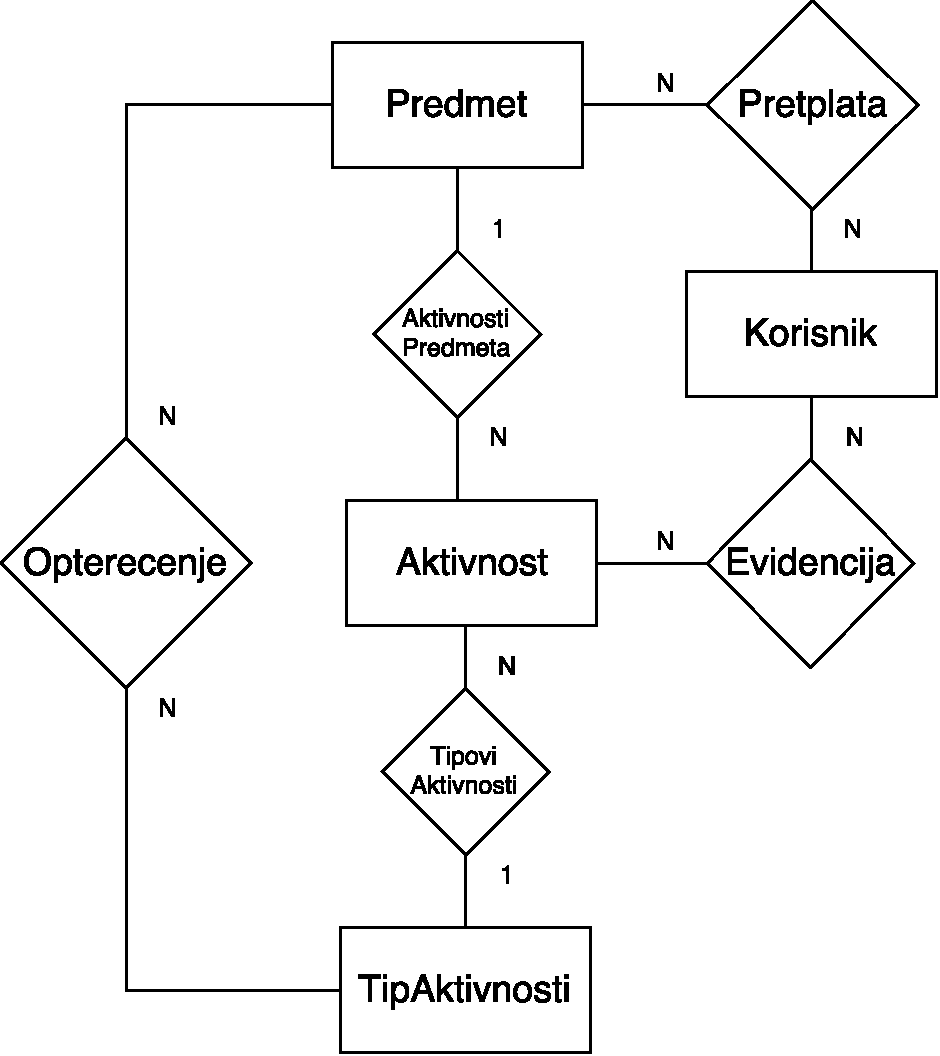
\includegraphics[scale=0.8]{img/er-model.pdf}
\caption{Konačni ER model}
\label{fig:er-model}
\end{figure}

\begin{figure}[H]
\centering
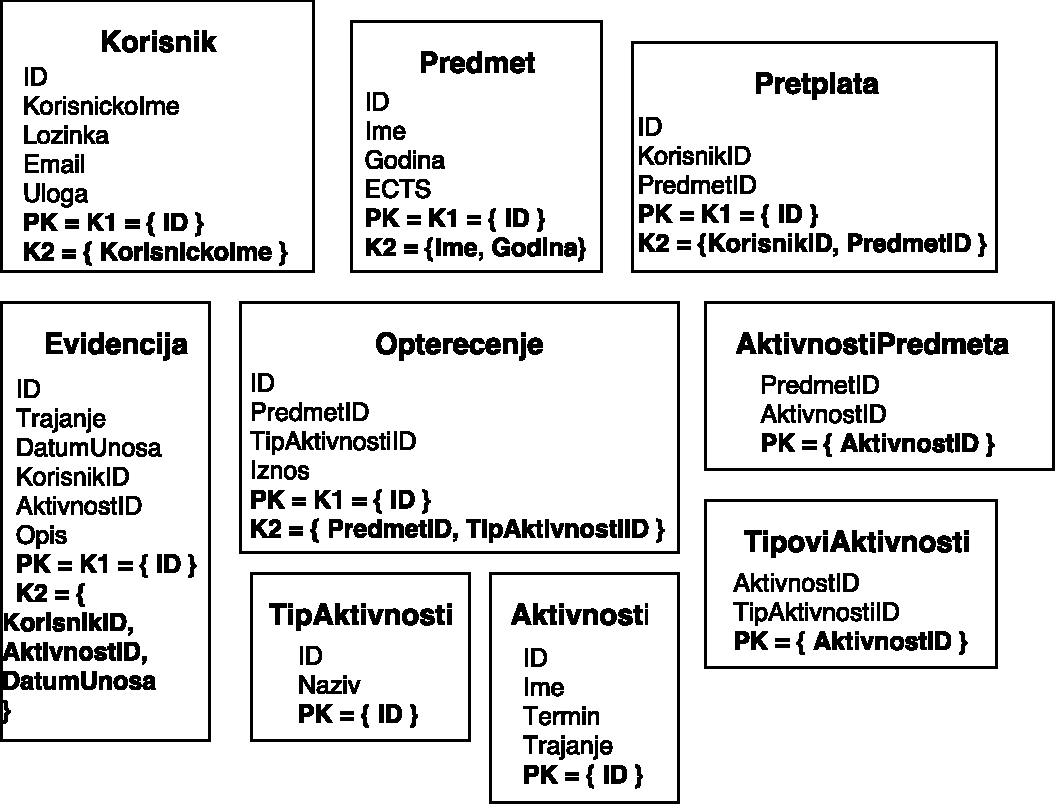
\includegraphics[scale=0.8]{img/er-model-opis.pdf}
\caption{Entiteti i veze}
\label{fig:er-model-opis}
\end{figure}

Svi postojeći kompozitni ključevi zamijenjeni su sa surogatnim ključevima radi lakšeg rada web aplikacije. U slučajevima poput veze 'Evidencija', kompozitni ključ samo donosi dodatna opterećenje u web aplikaciju - prilikom svakog dohvata evidencije potrebno je pretraživati po svim troje vrijednostima (KorisnikID, AktivnostID i DatumUnosa), a tijekom komunikacije između poslužitelja i klijenta putem Ajax-a trebaju se prenositi sve troje vrijednosti, dok sami kompozitni ključ ne donosi u ovom slučaju ikakve prednosti. Prirodni ključevi ostalih entiteta i veza zamijenjeni su surogatnim ključevima zbog istih razloga ili radi konzistentnosti.

\section{Relacijski model}

ER konceptualni model koristan je za grafički prikaz baze podataka i opis veza između entiteta. Međutim, stvarne baze podataka koje koriste web aplikacije (poput ove) su opisane relacijskom shemom. Zato se ER model pretvara u relacijski čime se dobiva sljedeća shema (razgranati krajevi veze označavaju višestrukost):

\subsection{Dijagram}

\begin{figure}[H]
\centering
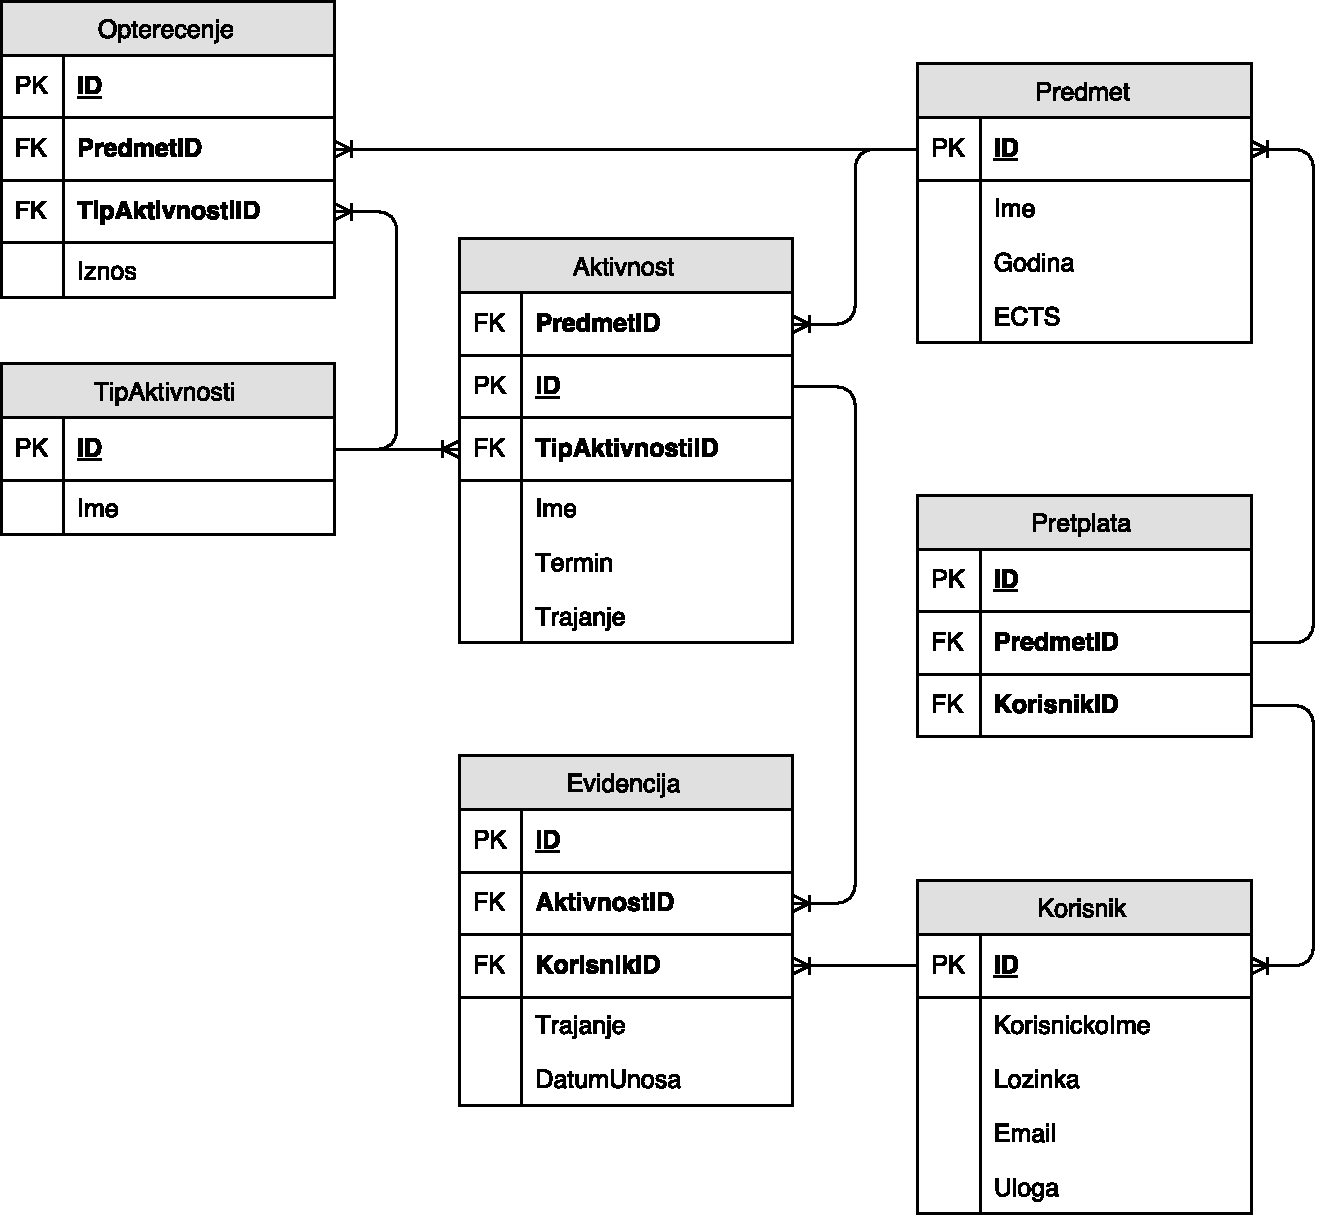
\includegraphics[scale=0.5]{img/relacijski-model.pdf}
\caption{Relacijski model}
\label{fig:relacijski-model}
\end{figure}

\subsection{SQL kod}

Za svaki primarni ključ dodatno je definirano ograničenje IDENTITY, kojim se u bazi definira da je atribut stvoren od strane baze podataka - prilikom unosa novih podataka unose se svi atributi osim atributa 'ID' pošto njega generira sama baza podataka, i to tako da kao vrijednost koristi inkrementiranu zadnju korištenu vrijednost tog atributa.

\lstset{style=sql, numbers=left}
\lstinputlisting{code/baza.sql}

\chapter{Web aplikacija}
\section{Alati i tehnologije}

\subsection{Entity Framework}

Entity Framework je skup ADO.NET tehnologija koje podržavaju razvoj podatkovno-orijentiranih aplikacija. Programeri takvih aplikacija tipično imaju potrebu realizirati 2 vrlo različita cilja: Moraju modelirati entitete, veze, i poslovnu logiku aplikacijskog sloja; te moraju raditi sa podatkovnim motorima \engl{data engine} koji dohvaćaju i ažuriraju podatke.

Entity Framework omogućuje programerima da rade sa podacima u obliku domenski specifičnih objekata, bez direktne komunikacije sa temeljnom bazom podataka gdje se ti podaci nalaze. Na ovaj način ostvaruje se viša razina apstrakcije koja omogućava brže stvaranje aplikacija i to sa manje koda.

Podloga Entity Framework-a su entiteti. Svaki entitet sadrži svojstva \engl{properties} koja ga definiraju. Svaki entitet ima barem jedan ključ koji ga unikatno određuje \engl{key property}. Svojstva općenito mogu biti jednostavni ili kompleksni podaci: jednostavni su primitive definirane .NET okvirom, dok su kompleksni bilo koje klase ili strukture definirane od strane korisnika. 
Moguće je izraziti odnose između entiteta preko asocijacija. Asocijacije su slične vezama ER modela - također određuju svojstva i kardinalnosti po kojima su entiteti međusobno povezani.

Da bi se omogućio pristup podacima jednog entiteta drugome, entiteti imaju navigacijska svojstva. Svaki entitet koje je asociran sa nekim drugim može preko navigacijskih svojstava direktno pristupiti svim podacima tog drugog entiteta, i obratno. Slična su stranim ključevima baze podataka, ali je lakše raditi s njima pošto se Entity Framework brine za većinu komunikacije sa bazom podataka.\clearpage

Sve informacije entiteta spremljene su u entitetskom kontejneru \engl{entity container}. Prije nego što se može vršiti interakcija nad entiteta potrebno je instancirati jedan kontejner. Ta instanca kontejnera naziva se kontekst \engl{context} i ona predstavlja trenutačno stanje baze podataka. Aplikacija tada pristupa i manipulira svim entitetima preko tog konteksta.

Entity Framework omogućuje stvaranje modela na 3 načina \citep{entity}:
\begin{enumerate}
\item \textbf{Baza prvo} \engl{Database first} pristupom Entity Framework generira model na osnovu već postojeće baze podataka koristeći obrnuto inženjerstvo \engl{reverse engineering}.
\item \textbf{Dizajn prvo} \engl{Design first} omogućuje grafičko 'crtanje' modela čime Entity Framework stvara novu bazu podataka koja odgovora modelu.
\item \textbf{Kod prvo} \engl{Code first} načinom ručno se piše sav kod koji definira model, nakon čega Entity Framework stvara bazu podataka koja odgovara modelu.
\end{enumerate}

Nakon što je stvoren model baze (na koji god način), inicijalizira se kontekst:

\lstset{style=csharp, numbers=none}
\lstinputlisting{code/context.cs}

Podacima se zatim može manipulirati pomoću LINQ izraza:

\begin{enumerate}
\item \textbf{Where} - Dohvaća sve n-torke relacije koje zadovoljavaju uvjet (lambda izraz) koji je naveden kao argument metode:

\lstinputlisting{code/where.cs}
\item \textbf{Select} - Mapiranjem pretvara dohvaćene podatke u drugi skup podataka:
\lstinputlisting{code/select.cs}
\item \textbf{Add} - Dodaje novu n-torku u bazu podataka:
\lstinputlisting{code/add.cs}
\item \textbf{Update} - Ažuriranje podataka vrši se dohvaćanjem i mijenjanjem atributa:
\lstinputlisting{code/update.cs}
\item \textbf{Remove} - Briše postojeći objekt iz baze:
\lstinputlisting{code/remove.cs}
\item \textbf{SaveChanges} - Sve promjene ne provode se odmah nakon poziva odgovarajućih metoda. Potrebno je pozvati metodu \emph{SaveChanges()} koja provodi sve promjene zabilježene u kontekstu nad bazom podataka (i baca odgovarajuće iznimke u slučaju greške):

\lstinputlisting{code/savechanges.cs}
\end{enumerate}

\subsection{ASP.NET MVC}

ASP.NET MVC (Active Server Pages .NET Model-View-Controller) je Microsoft-ov okvir za izradu web aplikacija koji ujedinjuje efektivnost i urednost MVC arhitekture, najnovije ideje i tehnike agilnog programiranja, te najbolje dijelove postojeće ASP.NET platforme kao alternativa tradicionalnim ASP.NET web formama \citep{mvc}.
	
Interakcije sa MVC (hr. model-pogled-upravljač) aplikacijom slijede prirodni ciklus korisničkih akcija i osvježavanja pogleda, gdje se za pogled podrazumijeva da ne pamti stanja. To se uklapa sa HTTP zahtjevima i odgovorima na kojima se temelji svaka web aplikacija. MVC razdvaja web aplikacija domene: domenu modela, upravljačke logike, te korisničkog sučelja, čime se HTML korisničkog sučelja odvaja od samih implementacijskih detalja aplikacije. 
MVC web aplikacija sastoji se od 3 glavna dijela:
\begin{enumerate}
\item \textbf{Modeli} -
Modeli sadržavaju ili opisuju podatke sa kojima korisnici rade. Oni mogu biti jednostavni modeli pogleda, koji predstavljaju podatke koji se prenose iz pogleda do upravljača i obratno; ili mogu biti domenski modeli, koji predstavljaju podatke poslovnog sloja kao i operacije koje se mogu vršiti nad njima. Odgovorni su za čuvanje trenutnog stanja i konzistentnosti podataka koje predstavljaju.

\item \textbf{Pogledi} -
Pogledi prikazuju dio ili cijeli model kao korisničko sučelje. Obuhvaćaju svu logiku potrebnu za prikaz elemenata modala ali ništa više. Osim prikaza, nisu svjesni postojanja modela te ne komuniciraju neposredno sa modelom na bilo koji način.

\item \textbf{Upravljači} -
Upravljači obrađuju dolazeće zahtjeve, vrše operacije nad model, te odabiru poglede kojima će se rezultat obrade prikazati korisniku. Oni su most između pogleda i modela, koji definira sve putove komunikacije klijenta i web aplikacije.\\
\end{enumerate}

\begin{figure}[H]
\centering
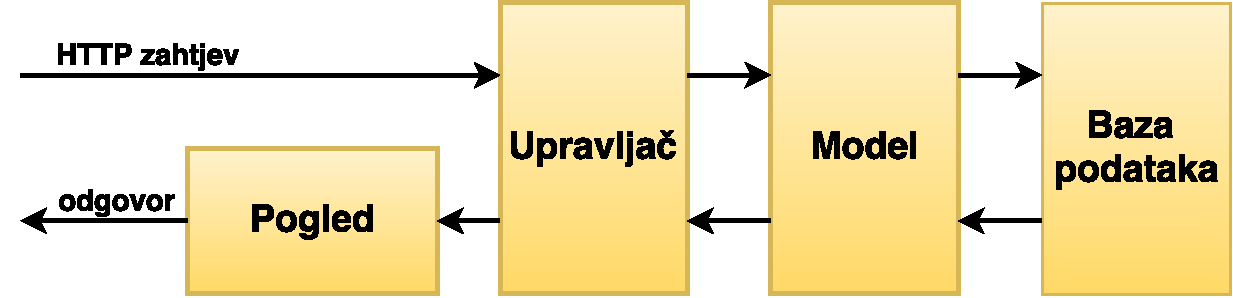
\includegraphics[scale=0.7]{img/mvc.pdf}
\caption{Relacijski model}
\label{fig:mvc}
\end{figure}

Svaki dio MVC arhitekture definiran je zasebno kao samostalna jedinka: logika koja mijenja model nalazi se samo u modelu, logika koja prikazuje podatke nalazi se samo u pogledu, a logika koja upravlja dolazećim korisničkim zahtjevima nalazi se samo u upravljaču - sa ovom razdiobom aplikacija se lakše održava i nadograđuje, pošto promjena koda u jednom dijelu neće imati direktne posljedice na ostatku aplikacije.

Za izradu ove web aplikacije koristi se ASP.NET MVC i to u sklopu razvojnog okruženja \emph{Visual Studio} koje osim izrade same web aplikacije pruža i potporu za korištenje prethodnog navedenog Entity Framework-a, koju ova web aplikacija koristi za komunikaciju sa bazom podataka. Upravljači i modeli napisani su u programskom jeziku C\# (C Sharp), dok je pogled napisan u html-u uz dodatno korištenje pomoćnih \emph{Razor} metoda koje omogućuju dinamičko kreiranje web stranica.\clearpage

\subsection{Ajax}

Ajax je način komuniciranja sa web poslužiteljem bez osvježavanja cijele stranice \citep{ajax}.
To je skup tehnologija koje omogućavaju dodatne funkcionalnosti u radu sa web aplikacijama:
\begin{enumerate}
\item Ažuriranje bez osvježavanja cijele web stranice.
\item Slanje podataka poslužitelju nakon učitavanja stranice.
\item Primanje podataka od poslužitelja nakon učitavanja stranice.
\item Pozadinsko slanje podataka poslužitelju.
\end{enumerate}

Na tradicionalnim web stranicama, preglednik \engl{browser} šalje zahtjev poslužitelju za cijelom stranicom. Tada, korisnik odabire poveznicu ili predaje formu čime preglednik šalje zahtjev poslužitelju, poslužitelj opet vraća cijelu stranica kao odgovor, te se ciklus nastavlja.

Ajax metodologija se udaljava od takvog načina rada. Kada korisnik vrši interakciju nad stranicom, preglednik šalje diskretne podatke. Umjesto da poslužitelj ponovno pošalje cijelu novu stranicu kao odgovor, on samo ažurira postojeću u odnosu na pristigle podatke.\\

\begin{figure}[H]
\centering
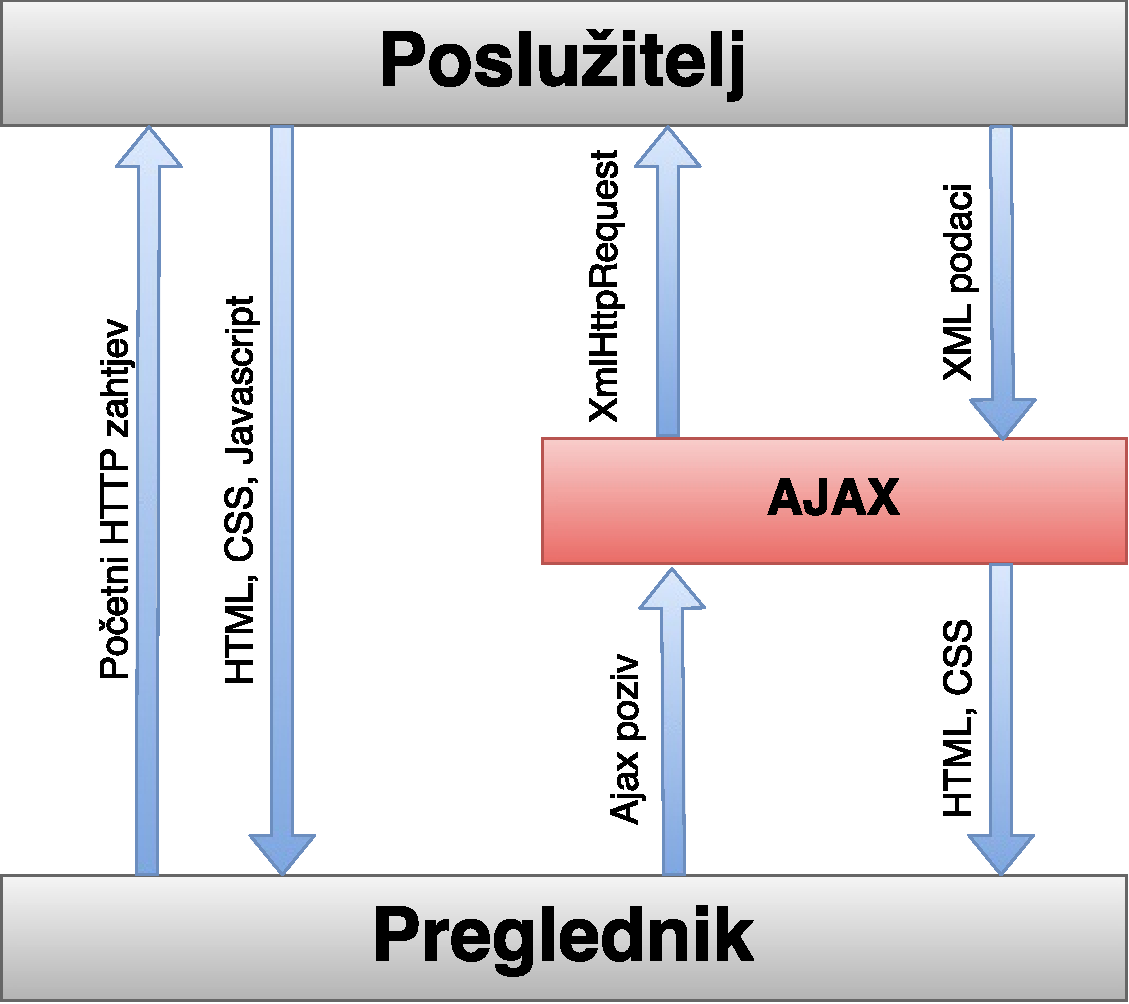
\includegraphics[scale=0.5]{img/ajax-dijagram.pdf}
\caption{Ajax dijagram}
\label{fig:ajax-dijagram}
\end{figure}
\clearpage
Slanje podataka ostvaruje se pozivom \emph{ajax()} funkcije, čiji najosnovniji poziv izgleda ovako (postoje mnoge druge opcije koje se mogu dodati):

\lstset{style=js, numbers=none}
\lstinputlisting{code/ajax.js}

Nakon uspješnog slanja zahtjeva, \emph{success} funkcija može pristupiti podacima koji su poslani od strane poslužitelja, te ažurirati web stranicu na koji god način je potrebno putem JavaScript-a.

\textbf{jQuery} je jedna od najpopularnijih JavaScript biblioteka danas u korištenju jer omogućava brzu i jednostavnu izgradnju web stranica i web aplikacija. Svrha jQuery-a je lakše korištenje JavaScript-a u web aplikacijama.\\

Mnogi česti zadaci koji zahtjevaju puno linija koda u JavaScript-u omataju se sa jedno linijskim jQuery funkcijama koje znatno ubrzavaju proces izrade web aplikacije. Tipični primjer je dohvaćanje elemenata:

Dohvaćanje elementa JavaScript-om,

\lstset{style=js, numbers=none}
\lstinputlisting{code/javascript.js}

i dohvaćanje sa jQuery-em:

\lstinputlisting{code/jquery.js}

Svojstva jQuery biblioteke \citep{jQuery}:
\begin{enumerate}
\item Efikasna HTML i CSS manipulacija
\item HTML događaji \engl{events}
\item Grafički efekti i animacije
\item Jednostavno korištenje Ajax-a
\item Kompatibilnost sa većinom preglednika
\item jQuery UI korisničko sučelje - kalendari, grafovi, tabovi, dijalozi, validacija...
\item Pomoćne funkcije koje nadograđuju postojeće JavaScript funkcionalnosti.
\end{enumerate}

U sklopu ove aplikacije osim pomoćnih jQuery funkcija za pronalazak elemenata DOM-a (Document Object Model), koristi se i jQuery funkcija \emph{post()}, koja je zapravo samo omotač oko običnog Ajax poziva:

\lstinputlisting{code/jquery-post.js}

Na ovaj način nakon svakog ažuriranja pretplate, evidentiranja utrošenog vremena, ili pregleda statistike, svi podaci web stranice koje je korisnik pohranio putem preglednika (dinamički generirani sadržaj poput grafova, trenutno odabrane postavke, itd.) ostaju pohranjeni, te se samo ažurira onaj dio stranice koji je izmjenjen. Time se komunikacija između klijenta i poslužitelja znatno ubrzava, pošto se ne šalju redundantni podaci putem mreže, a i znatno olakšava, pošto klijent pamti stanje web stranice tijekom komunikacije sa poslužiteljem.\clearpage

\section{Implementacija}
\subsection{Prijava}
Da bi korisnik uopće mogao koristiti bilo koji dio aplikacije, treba se prvo prijaviti u sustav putem korisničkog računa, kao što to obično jest u većini slučajeva kada god su u pitanju web aplikacije. Potrebno je implementirati barem najosnovniji dio sustava za prijavu, kako bi se sve evidencije mogle povezati sa svojim odgovarajućim korisnicima. Na ovaj način korisnik može tijekom pregleda statistike vidjeti zasebno svoju statistiku (izračunatu temeljem njegovih evidencija), a zasebno sve ostalo.

\begin{figure}[H]
\centering
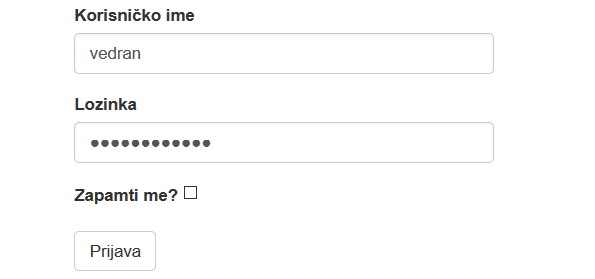
\includegraphics[scale=0.7]{img/prijava.png}
\caption{Prijava}
\label{fig:prijava}
\end{figure}

Stranica za prijavu sastoji se od polja za unos korisničkog imena i polja za unos lozinke, gdje korisnik upisuje svoje korisničke podatke. Nakon unosa podataka korisnik odabire tipku 'Prijava' čime se šalje zahtjev za autentifikaciju. Server tada uzima korisničko ime od klijenta te provjerava da li navedeni korisnik usitinu postoji u bazi podataka. Ako korisničko ime ne postoji, klijentu se ispisuje odgovarajuća greška. Ako postoji, to znači da u bazi postoji n-torka u relaciji 'Korisnik' koja sadrži sve korisnikove podatke, uključujući i njegovu kriptiranu lozinku. Lozinka koju je korisnik unio prilikom prijave sada se enkriptira te se uspoređuje sa lozinkom pohranjenom u bazi.

\lstset{style=csharp}
\lstinputlisting{code/prijava.cs}

Ako su jednake, autorizacija uspijeva te korisnik biva prijavljen, nakon čega ga se preusmjerava na stranicu za odabir predmeta. U slučaju pogreške ispisuje se odgovarajuća greška: nepostojeće korisničko ime, ili pogrešna lozinka.

Prilikom prijave moguće je označiti dodatnu opciju 'Zapamti me?'. Bez te opcije, nakon prijave, korisnik će nakon jedog vremenskog perioda neaktivnosti biti automatski odjavljen. Sa tom opcijom, serveru se daje do znanja da zapamti korisnika i da ga ne odjavi nakon navedenog vremenskog perioda, nega da ga zapamti dokle god se u 'kolačićima' klijentovih zahtjeva nalazi identifikator sjednice \engl{session id}.

U slučaju da korisnik nema već postojeći račun na koji se može prijaviti, postoji i mogućnost registracije novog korisničkog računa:

\begin{figure}[H]
\centering
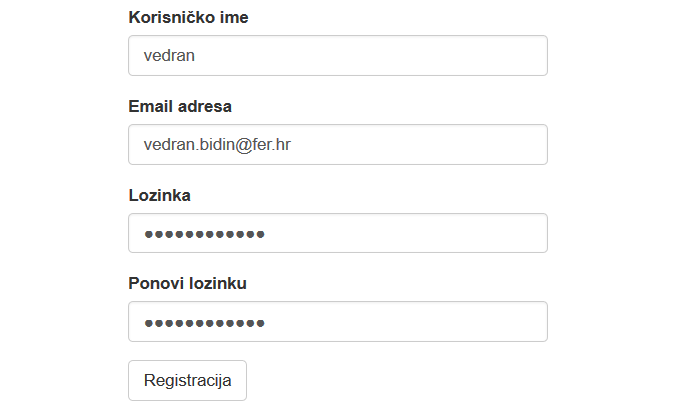
\includegraphics[width=\textwidth,height=\textheight,keepaspectratio]{img/registracija.png}
\caption{Registracija}
\label{fig:registracija}
\end{figure}

Kao što je vidljivo iz slike, potrebno je unesti osnovne podatke: korisničko ime, email adresu, te lozinku. U slučaju da navedeno korisničko ime već postoji u bazi, registracija neće biti moguća, pošto korisnička imenu moraju biti unikatna. Lozinku je potrebnu unesti dva puta, kako bi se smanjila mogućnost registracije sa pogrešno unesenom lozinkom.

Prijava i registracije oboje se provode koristeći klasični HTTP POST zahtjev, čija se obrada znatno olakšava korištenjem modela:
Model je obični razred koji sadrži neki broj polja, koja mogu biti bilo kojih tipova. Za svako polje mogu biti definirani određeni atributi, koji postavljaju dodatna ograničenja (da li polje nužno mora biti uneseno, da li mora sadržavati barem N znakova, i slično):

\lstset{style=csharp}
\lstinputlisting{code/registracija-model.cs}

Na početku pogleda (na prvoj liniji) deklarira se put do modela:

\lstset{style=html}
\lstinputlisting{code/model.cshtml}

Tada se u pogledu definiraju elementi koji odgovaraju podacima iz modela. Za sve podatke koje je potrebno unesti, postavljaju se odgovarajući \emph{input} elementi (koji mogu biti tekstovna polja, gumbi, padajuće liste i slično) koji služe za pohranu unesenih korisnikovih podataka te napokon \emph{submit} tipka čijom pritiskom se šalje POST zahtjev. Svi elementi se dodatno enkapsuliraju sa \emph{form} elementom, čime se podaci koji sadrže šalju zajedno sa POST zahtjevom.

\lstset{style=html}
\lstinputlisting{code/registracija-view.cshtml}

\clearpage
Zatim se u upravljaču koji prima HTTP zahtjev kao jedan od parametara dodaje prethodno definirani model, čime se tijekom svake obrade zahtjeva može podacima iz forme na jednostavan način pristupiti preko parametra koji predstavlja taj model:

\lstset{style=csharp}
\lstinputlisting{code/registracija-cont.cs}

\subsection{Pretplata}
Nakon što je korisnik prijavljen, on može evidentirati te pregledavati svoje utrošeno vrijeme. Međutim, kako se sve evidencije zapravo vežu uz određeni predmet, evidentiranje i pregled se izvršavaju u odnosu na jedan od mnogih dostupnih predmeta. Zato korisnik uvijek prije evidencije odnosno pregleda mora odabrati jedan od tih predmeta. Kako broj predmeta može biti poprilično velik, korisnik bi prije svake evidencije i pregleda morao tražiti od svih mogućih predmeta onaj za koji želi evidentirati odnosno pregledavati statistiku. Zato je korisniku omogućena pretplata na predmet:

\begin{figure}[H]
\centering
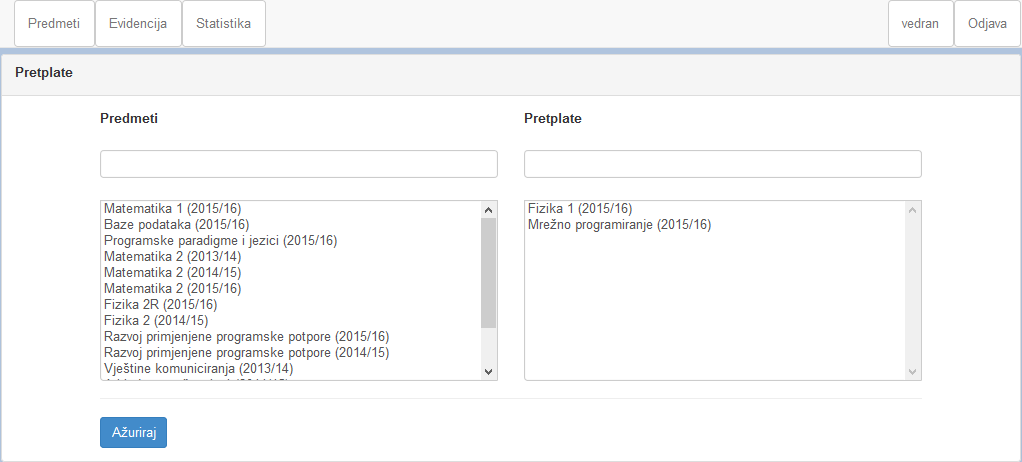
\includegraphics[width=\textwidth,height=\textheight,keepaspectratio]{img/pretplata-web.png}
\caption{Pretplata}
\label{fig:pretplata-web}
\end{figure}
\clearpage

U ovom dijelu trenutno prijavljeni korisnik može definirati na koje predmete želi biti pretplaćen. U lijevoj listi nalaze se svi dostupni predmeti, a u desnoj listi se nalaze svi pretplaćeni predmeti. Korisnik može selekcijom na bilo koje od predmeta ili bilo koje grupe predmeta dodavati odnosno brisati odgovarajuće pretplate. \\

\textbf{Bootstrap Dual Listbox} (http://www.virtuosoft.eu/code/bootstrap-duallistbox/)\\
Popisi pretplaćenih i nepretplaćenih predmeta ostvareni su pomoću Bootstrap Dual Listbox plugin-a koji omogućava lagano upravljanje dvojnom listom. U pogledu za pretplate definira se \emph{select} element, nad kojim se tijekom učitavanja stranice poziva funkcija \emph{bootstrapDualListbox()} sa pripadajućim opcijama:

\lstset{style=js}
\lstinputlisting{code/duallistbox.js}

Nakon svih izmjena, pritiskom na tipku 'Ažuriraj' provode se sve promjene te se ažurira popis pretplata odabrane od strane korisnika. Nakon toga u ostalim dijelovima web aplikacije korisnik na raspolaganju za odabir ima samo predmete na koje se unutar ove stranice pretplatio.

Ako se slanje novih pretplaćenih predmeta radi klasničnim POST zahtjevom, cijela stranica nakon ažuriranja se ponovno učitava, kako je to i inače slučaj sa običnim POST zahtjevima. Međutim, poželjno je ažurirati popis pretplaćenih predmeta bez ponovnog učitanja cijele stranice, jer to podrazumijeva ponovno čitanje svih predmeta iz baze podataka, što nepotrebno troši vrijeme poslužitelja, pošto su svi predmeti već bili učitani prilikom prvog otvaranja stranice.

Zato se slanje ažuriranih pretplata radi korištenjem Ajax-a. Definira se funkcija koja se poziva tijekom pritiska tipke 'Ažuriraj', koja prvo iz liste predmeta pronalazi sve one na koje je korisnik pretplaćen te ih sprema u polje koje sadrži njihove identifikatore. Zatim se koristi jQuery funkcija \emph{post()} (koja je omotač oko poziva funkcije \emph{ajax()}) koja prosljeđuje navedene identifikatore pretplaćenih predmeta poslužitelju:
\clearpage

\lstset{style=js}
\lstinputlisting{code/pretplate-ajax.js}

Upravljač tada na osnovi dobivenih identifikatora, odnosno primarnih ključeva predmeta, ažurira korisnikove pretplaćene predmete.

Pošto broj predmeta može biti velik, dodatno na vrhu svakih od listi nalazi se polje za filtriranje. U to polje može se unesti niz znakova (dio ili cijeli naziv predmeta) nakon čega se lista odmah ažurira, te prikazuje samo one predmete koje sadrže navedeni niz znakova:

\begin{figure}[H]
\centering
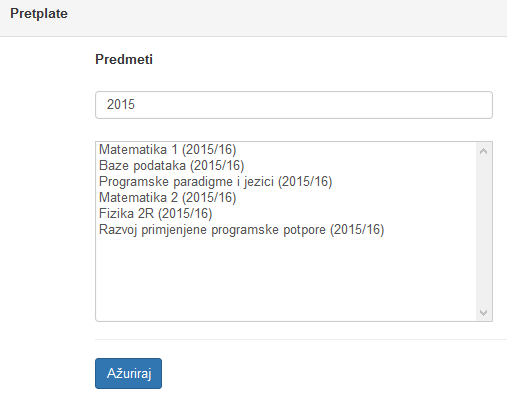
\includegraphics[scale=0.85]{img/filtriranje.png}
\caption{Filtriranje predmeta po godini}
\label{fig:filtriranje}
\end{figure}
\clearpage

\subsection{Evidencija}
Ovaj dio web aplikacije omogućava prijavljenim korisnicima da evidentiraju svoje utrošeno vrijeme za predmete na koje su pretplaćeni:

\begin{figure}[H]
\centering
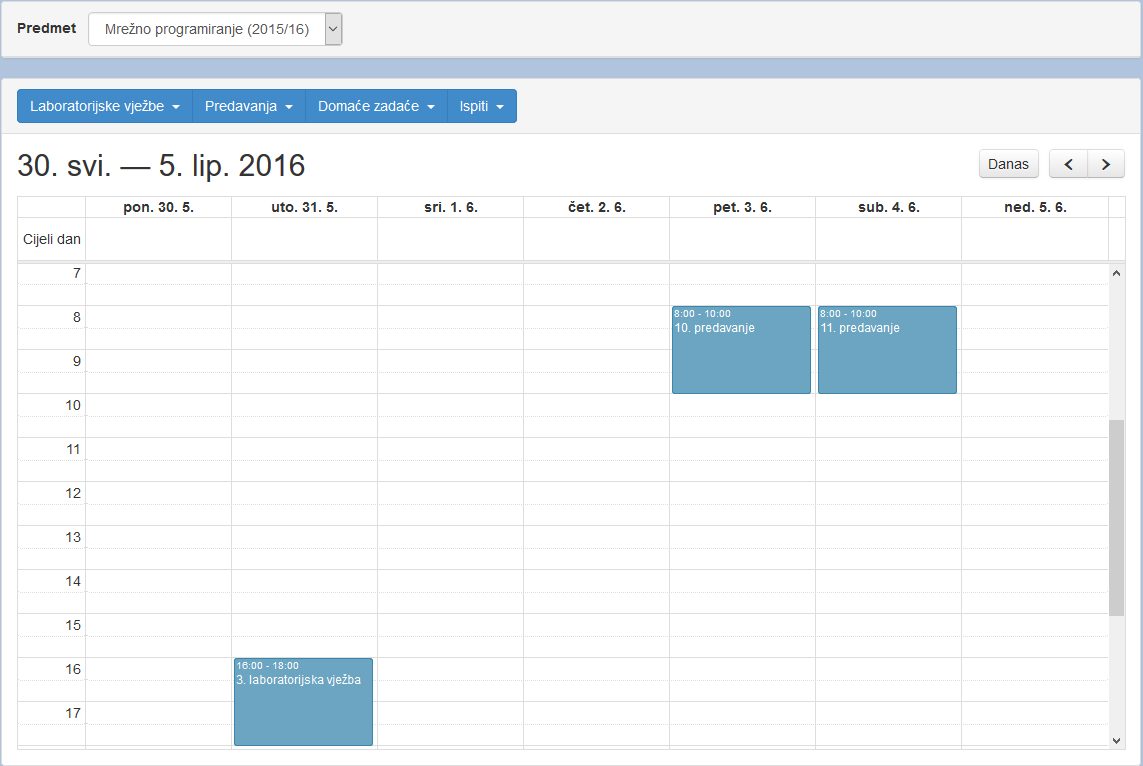
\includegraphics[width=\textwidth,height=\textheight,keepaspectratio]{img/evidencija-web.png}
\caption{Evidentiranje predmeta}
\label{fig:evidencija-web}
\end{figure}

Evidencija se sastoji od 3 dijela:

\begin{enumerate}[leftmargin=*]
\item Na vrhu je padajuća lista koja sadrži sve pretplaćene predmete trenutno prijavljenog korisnika. Ovdje korisnik odabire predmet za koji želi evidentirati utrošeno vrijeme.

\item \textbf{Izbornik aktivnosti}\\
Nakon što korisnik odabere jedan od njegovih pretplaćenih predmeta putem padajuće liste, ova stranica putem Ajax-a dinamički se ažurira sa svim novim aktivnostima toga predmeta: upravljaču se šalje identifikator predmeta, nakon čega on dohvaća sve aktivnosti iz baze podataka koje pripadaju odabranome predmetu te ih vraća pogledu, koji ažurira tipove aktivnosti izbornika tako da odgovaraju svim tipovima aktivnosti odabranoga predmeta, nastanjuje ih sa odgovarajućim aktivnostima, te ažurira kalendar sa svim aktivnostima koji imaju definiran termin.
\clearpage

\textbf{FullCalendar} (http://fullcalendar.io/)\\
FullCalendar je jQuery plugin koji omogućava prikazivanje kalendara. Pruža veliki raspon mogućnosti: prikazivanje po mjesecu, tjednu, danu, interaktivnost kalendara (stvaranje novih termina, ažuriranje postojećih), dinamičko mijenjanje sadržaja kalendara putem Ajax zahtjeva, i mnoge druge mogućnosti koje se u ovoj web aplikaciji ne koriste. FullCalendar koristi službena stranica \emph{fer.hr} za prikaz termina predmeta i dvorana putem kalendara.

\lstset{style=js}
\lstinputlisting{code/kalendar.js}

Aktivnosti su podijeljene prema tipu aktivnosti: odabirom jednog od tipova aktivnosti otvara se nova padajuća lista koja sadrži sve aktivnosti toga tipa. Naprimjer ako se za predmet 'Mrežno programiranje' odabere tip aktivnosti 'Predavanja', stranica bi mogla izgledati ovako:

\begin{figure}[H]
\centering
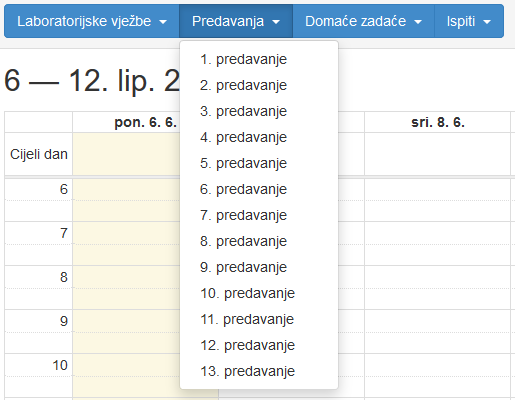
\includegraphics[scale=0.8]{img/selekcija.png}
\caption{Odabir tipa aktivnosti}
\label{fig:selekcija}
\end{figure}
\clearpage

Nakon što je odabran tip aktivnosti, korisnik ima pregled svih aktivnosti toga tipa, te tada odabire jednu od tih aktivnosti, onu za koju želi evidentirati utrošeno vrijeme. Nakon odabira aktivnosti otvara se novi modalni prozor:

\begin{figure}[H]
\centering

\includegraphics[width=\textwidth,height=\textheight,keepaspectratio]{img/modal.png}
\caption{Unos utrošenog vremena}
\label{fig:modal}
\end{figure}

Modalni prozor sastoji se od polja u koje se unosi iznos utrošenog vremena, i padajuće liste u kojoj se odabire mjerna jedinica utrošenog vremena (minute ili sati). Nakon što korisnik unese podatke, odabere se opcija spremi čime se vrši validacija. U slučaju pogreške unosa podataka, naprimjer ako se umjesto iznosa vremena unese riječ ili slično, korisniku se ispisuje odgovarajući tekst pogreške. Ako je validacija prošla, unos se trajno pohranjuje u bazu, nakon čega se kao i sve ostale pohranjene evidencije koristi prilikom računanja statistike koja je dostupna na stranici imena 'Statistika'. 

\lstset{style=js}
\lstinputlisting{code/evidencija-spremi.js}

U slučaju pogreške od strane korisnika, modalni prozor može se ugasiti pritiskom na 'x' gumb u gornjem desnom kutu prozora čime se evidentiranje za tu specifičnu aktivnost otkazuje. Bez obzira na rezultat evidencije, korisnik opet može proizvoljno odabirati i evidentirati aktivnosti koliko god je potrebno.
\clearpage

\item \textbf{Kalendar}\\
Osim prethodno navedenog načina evidentiranja (odabirom aktivnosti putem izbornika), korisniku se dodatno omogućuje i evidentiranje putem kalendara. Sve aktivnosti odabranoga predmeta koje imaju u bazi definiran datum početka i/ili trajanje, mogu se vidjeti na kalendaru, ukoliko su to aktivnosti trenutno odabranoga predmeta. Korisnik može pregledavati sve aktivnosti putem kalendara, te ih aktivirati pritiskom na njih. Nakon takvog odabira, opet se otvara isti modalni prozor kao i prilikom klasičnog evidentiranja. Važno je napomenuti da neke aktivnosti nemaju definiran datum početka. U tom slučaju te aktivnosti se očito nemogu aktivirati putem kalendara, već se moraju odabrati putem izbornika.

FullCalendar interno podržava interaktivnost grafa, nakon pritiska na jedan od termina poziva se funkcija \emph{eventClick} koju se može proizvoljno definirati:

\lstset{style=js}
\lstinputlisting{code/kalendar-click.js}

\end{enumerate}

\subsection{Statistika}
Ovaj dio web aplikacije omogućava prijavljenim korisnicima da pregledavaju svoje trenutačno utrošeno vrijeme, te da ga uspoređuju sa drugim korisnicima kao i sa definiranim očekivanim utrošenim vremenom. Kao i kod drugih dijelova aplikacije, korisnik mora biti prijavljen na sustav. Korisnik ima na raspolaganju dvije kartice, prva od kojih omogućuje sljedeći pregled:

\begin{figure}[H]
\centering
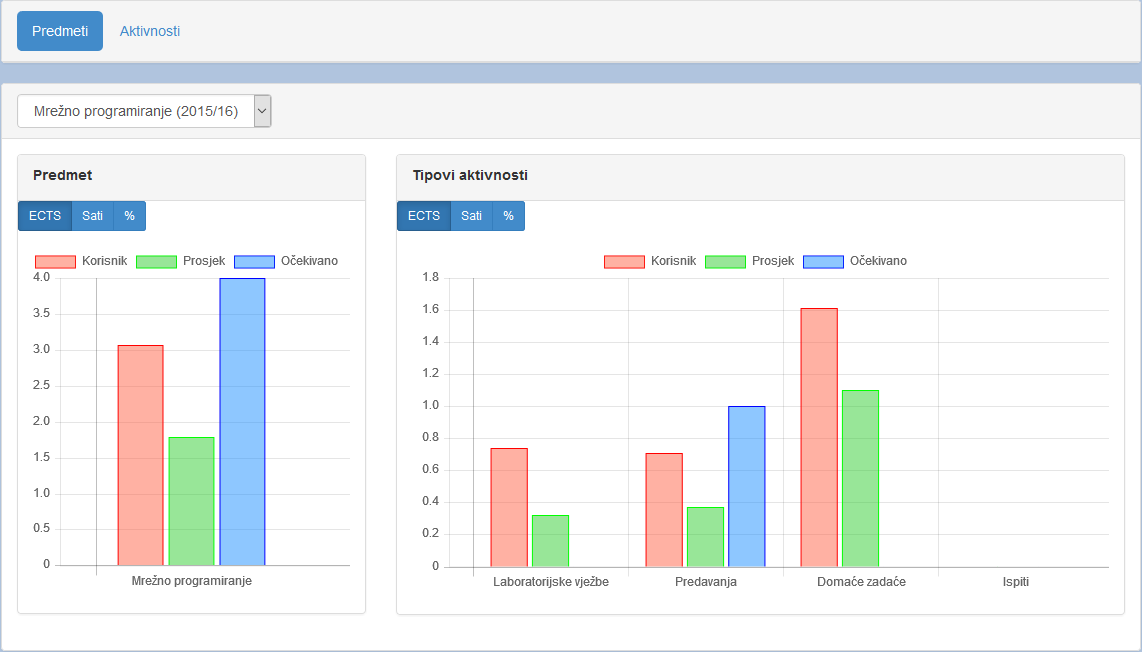
\includegraphics[width=\textwidth,height=\textheight,keepaspectratio]{img/statistika-web.png}
\caption{Statistika - kartica Predmeti}
\label{fig:statistika-web}
\end{figure}

Korisnik ovdje može odabrati jedan od predmeta na koje je trenutačno pretplaćen. U slučaju da predmet koji korisnik želi pregledavati nije na ovom popisu, potrebno je u izborniku 'Predmeti' pretplatiti se na taj predmet, nakon čega će on postati vidljiv u padajućoj listi.

Nakon odabira predmeta, odmah se ažurira statistika predmeta, tipova aktivnosti, te i samih aktivnosti. Korisnik ima na raspologanja 3 grafa. Prvi graf 'Predmet' omogućuje korisniku pregled utrošenog vremena na razini cijelog predmeta, odnosno obuhvaća ukupan iznos utrošenog vremena. Sve evidencije koje je korisnik ikada evidentirao za trenutačno navedeni predmet bit će prikazane u obliku stupčastog \engl{bar} grafa u trenutno odabranim mjernim jedinicama. Osim samih korisnikovih podataka, također su i na raspolaganju drugi podaci: jedan od njih je prosjek utrošenog vremena svih evidencija za taj predmet. Pod time se zapravo misli na prosjek ukupnog utrošenog vremena svih korisnika koji su ikada evidentirali ovaj predmet.

Osim tog podatka, također postoji i iznos ECTS bodova koji je definiran za svaki predmet prilikom njegovog unosa. Sa ECTS bodovima može se izračunati očekivani utrošak vremena za taj predmet, pošto vrijedi da jedan ECTS bod iznosi ~28 sati. Korisnik može vidjeti koliko je vremena utrošio on, koliki je prosjek utrošenog vremena, te koliko je vremena 'trebalo' (otprilike) biti utrošeno. To je korisna informacija koja može pokazati koliko je dobro definiran predmet: da li uzima manje vremena nego što bi trebao, više nego što bi trebao, te u kojim iznosu prekoračuje očekivano vrijeme.

\begin{figure}[H]
\centering
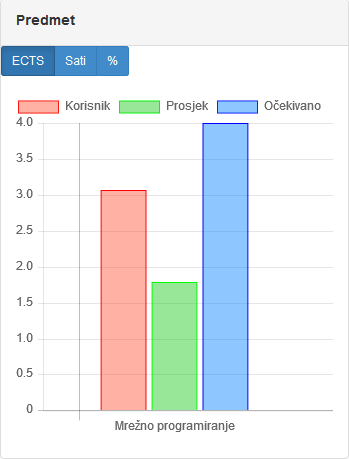
\includegraphics{img/statistika-predmet.png}
\caption{Statistika - predmet}
\label{fig:statistika-predmet}
\end{figure}

Sami podaci grafa dohvaćaju se korištenjem Ajax-a: nakon svakog odabira novog predmeta, poziva se funkcija koja uzima identifikator trenutačno odabranoga predmeta iz padajuće liste, te ga šalje odgovarajućem upravljaču:

\lstset{style=js}
\lstinputlisting{code/predmeti-change.js}

Upravljač tada izračunava svu statistiku vezanu uz sami predmet, te ju vraća u obliku JSON-a (JavaScript Object Notation). Nakon dobivene statistike za predmet, ponovno se šalje novi zahtjev, ovaj puta za trenutno odabranu aktivnost, koji onda vraća svu statistiku vezanu uz odabranu aktivnost toga predmeta.
\clearpage

U slučaju da je korisnik odabrao novi predmet, nakon dohvata statistike predmeta implicitno se dohvaća i statistika aktivnosti, pošto svaki predmet ima svoje zasebne aktivnosti koje je potrebno osvježiti. Međutim, u slučaju odabira nove aktivnosti (unutar kartice 'Aktivnosti'), ne dohvaća se statistika predmeta, već samo statistika te odabrane aktivnosti, pošto statistika predmeta ostaje nepromijenjena.

Odabir mjernih jedinica funkcionira na jednak način; jedina razlika je što se tijekom slanja Ajax zahtjeva zajedno sa zahtjevom šalje i niz znakova koji predstavlja mjernu jedinicu za koju je potrebno izračunati statistiku (ECTS bodovi, odnosno sati), koju upravljač prilikom stvaranja statistike uzima u obzir.

\lstset{style=js}
\lstinputlisting{code/aktivnosti-change.js}

Osim pregleda ukupno utrošenog vremena, korisnik također može pregledavati utrošeno vrijeme po tipovima aktivnosti koji su definirani za trenutačno odabrani predmet. Naprimjer, ako korisnik odabere predmet 'Mrežno programiranje', mogla bi se prikazati sljedeća slika:

\begin{figure}[H]
\centering
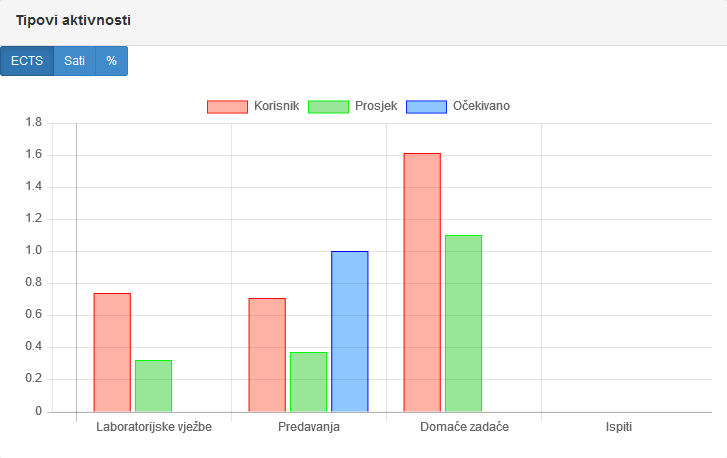
\includegraphics[scale=0.7]{img/statistika-tip-aktivnosti.png}
\caption{Statistika - tipovi aktivnosti}
\label{fig:statistika-tip-aktivnosti}
\end{figure}

Stupčasti graf sadrži iste 3 komponente kao i graf predmeta: iznos utrošenog vremena korisnika, prosječno utrošeno vrijeme, te očekivano utrošeno vrijeme (ukoliko postoji). Iznosi ovih komponenti definirani su za svaki tip aktivnosti trenutno odabranog predmeta. U slučaju tipa aktivnosti kao što su 'predavanja', u sklopu predmeta može biti definirano semestralno opterećenje sa određenim iznosom, koje određuje koliko vremena bi trebalo biti utrošeno za taj tip aktivnosti. To vrijeme se tada može direktno prikazati u grafu, čime se može vidjeti odstupanje od očekivane vrijednosti. Osim slučaja gdje je trajanje nekog tipa aktivnosti službeno definiran, očekivani utrošak vremena može se definirati 'ručno', za bilo koji tip aktivnosti, čime se može sustavu dati do znanja koliko bi vremena trebalo biti utrošeno za taj tip aktivnosti. Isto tako, moguće je da očekivano vrijeme ne postoji ili nije definirano, u kojem slučaju ono neće biti ni prikazano.

Ova statistika također prikazuje zanimljive podatke. Pregled utrošenog vremena po predmetu korisnicima daje opći pogled na predmet, dok sa sa ovom statistikom ulazi jedan sloj dublje: sada je dostupan pregled utrošenog vremena po tipu aktivnosti. Sa ovim pogledom moguće je vidjeti na koji način je raspodijeljeno utrošeno vrijeme: da li premalo ljudi ide na predavanja, da li laboratorijske vježbe oduzimaju previše vremena, da li su domaće zadaće previše lagane i slično.

Još postoji i treći graf: iznos utrošenog vremena po aktivnostima. Kada se odabere drugi izbornik, sučelje izgleda otprilike kao na slici:

\begin{figure}[H]
\centering
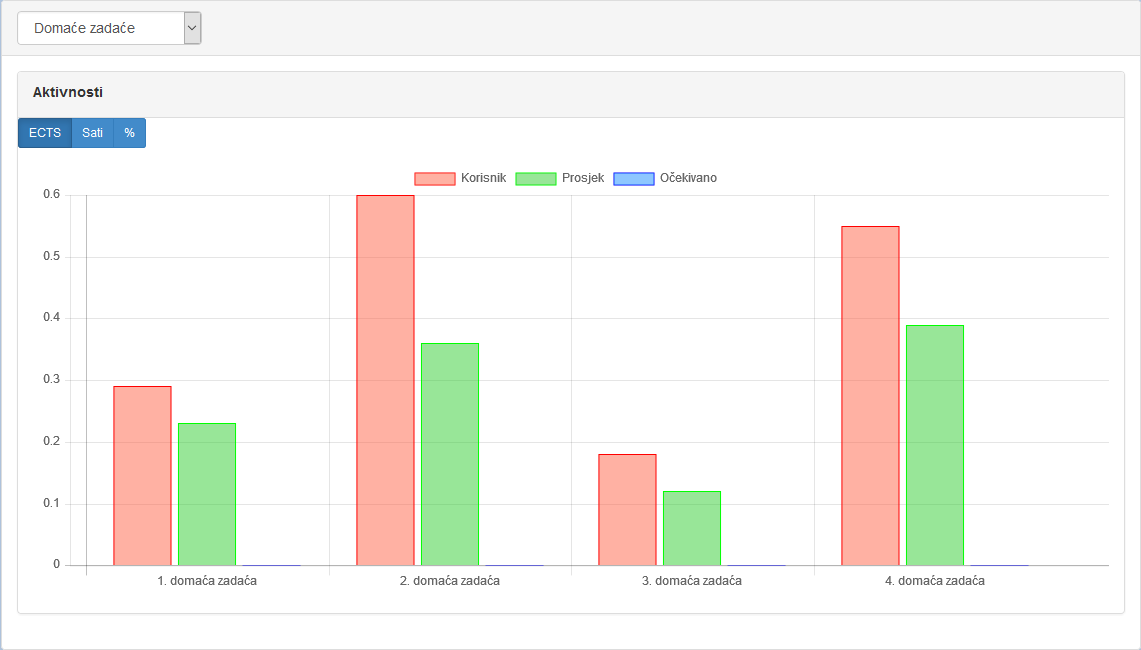
\includegraphics[width=\textwidth,height=\textheight,keepaspectratio]{img/statistika-aktivnosti.png}
\caption{Statistika - aktivnosti}
\label{fig:statistika-aktivnosti}
\end{figure}

Kao i na prijašnjoj stranici, na vrhu se nalazi padajuća lista. Međutim, sada padajuća lista sadrži sve tipove aktivnosti, i to sve tipove aktivnosti trenutačno odabranog predmeta na stranici 'Predmet'. Nakon odabira novog predmeta na prethodnoj kartici, ova padajuća lista odmah se osvježava, sa novim vrijednostima koje odgovaraju odabranom predmetu. Korisnik može izabrati jedan od ponuđenih tipova aktivnosti. Prilikom izbora novog tipa aktivnosti, dohvaćaju se sve aktivnosti koje su tog tipa, i koje pripadaju prethodno odabranome predmetu, zajedno sa svim njihovim evidencijama, te se grafički predočuje iznos utrošenog vremena po specifičnoj aktivnosti. Sa ovim grafom najdetaljnije se predočuje utrošeno vrijeme: može se vidjeti točno koliko je vremena utrošeno na pojedinačnu aktivnost što isto može biti korisna informacija.

Naprimjer, ako se pregledavaju sve laboratorijske vježbe određenoga predmeta, može se vidjeti koliko je vremena utrošena na jednu laboratorijsku vježbu, što je već samo po sebi dovoljan razlog za pregled ovog grafa. Međutim također se može vidjeti koliko je vremena utrošeno na specifičnu laboratorijsku vježbu (odnosno bilo koju aktivnost) u odnosu na druge aktivnosti. Time se može naprimjer uočiti da je određena laboratorijska vježba oduzela premalo vremena s obzirom na druge laboratorijske vježbe, ili da je priprema za laboratorijsku vježbu preteška s obzirom na samu laboratorijsku vježbu ili na druge pripreme.

Osim samog iznosa utrošenog vremena za korisnika i za prosjek, za svaku aktivnost u bazi podataka može biti evidentirano trajanje te aktivnosti. U slučaju primjerice predavanja to trajanje doslovce predstavlja predefinirani iznos trajanja predavanja određenog termina kao što je određeno po predmetu. Međutim, za aktivnosti koji nemaju već strogo definirana trajanja moguće je prilikom unosa aktivnosti definirati 'očekivano' trajanje, koje korisnicima daje do znanja koliko je vremena otprilike trebalo biti potrebno, ili koliki je očekivani utrošak vremena za tu aktivnost. U svakom slučaju, ako ta vrijednost nije poznata, ili čak nije ni važna, nije ju potrebnu ni unesti, pa će ta vrijednost tada ovdje biti neprikazana.
\clearpage

\textbf{Chart.js} (http://www.chartjs.org/)\\
Za prikaz grafova koristi se Chart.js, koji dodaje funkcionalnost crtanja dinamičkih interaktivnih grafova. Za svaki graf u pogledu se definira \emph{canvas} element, sa pripadajućom dužinom i širinom grafa,

\lstset{style=html}
\lstinputlisting{code/canvas.cshtml}

nad kojim se prilikom odabira novog predmeta ili aktivnosti, odnosno učitavanja nove statistike, konstruira novi graf:

\lstset{style=js}
\lstinputlisting{code/chart.js}
\clearpage

\section{Razvoj i poboljšanje}

\begin{enumerate}[leftmargin=*]
\item \textbf{Unos predmeta} - 
Trenutačno, kada je potrebno unositi nove predmete i/ili aktivnosti u bazu, potrebno je to učiniti preko direktne komunikacije sa bazom, koristeći naprimjer Visual-Studio ili SQL Server Management Studio. Iako to funkcionira, bilo bi korisno moći manipulirati tim podacima direktno preko korisničkog sučelja u samoj web aplikaciji. 

Na stranici predmet mogao bi se dodati gumb koji bi bio vidljiv samo administratorima, a koji bi otvarao novi modal u kojem se definiraju svi podaci predmeti, uključujući i tipove aktivnosti koje oni obuhvaćaju, kao i opterećenje predmeta.

Na stranici evidencije moglo bi se omogućiti dodavanje novih aktivnosti predmeta: FullCalendar omogućava interakciju sa kalendarom, pritisak na kalendar može se detektirati automatskim pozivom funkcije \emph{eventClick()} nakon čega bi se mogao otvoriti modal u kojem se mogu unijeti odgovarajući podaci aktivnosti, sa pretpostavljenim datumom početka koji odgovara pritisnutoj poziciji na kalendaru, te pohraniti novu aktivnost na kalendar putem funkcije \emph{renderEvent()}, dok se novu aktivnost u bazu može spremiti koristeći Ajax.

\item \textbf{Administracija} - 
Ne postoji korisničko sučelje aplikacije preko kojeg se privilegije korisnika mogu mijenjati. Bilo bi korisno implementirati sučelje preko kojeg korisnici sa administratorskom ulogom mogu pregledavati sve trenutne korisnike te im mijenjati njihove uloge, kao i onemogućiti im daljne aktivnosti nad aplikacijom (u slučaju da rade 'zle' stvari).

\item \textbf{Hijerarhija aktivnosti} - 
Trenutna organizacija aktivnosti u bazi podataka je dovoljna za potrebe evidentiranja većine predmeta, pogotovo jer same evidencije vrše studenti, koji nisu previše entuzijastični u vezi većine studentskih aktivnosti. Međutim, moguće je da se za neke aktivnosti želi evidentirati određene dijelove. Hipotetski, aktivnost '1. domaća zadaća' mogla bi se sastojati od 3 zadatka, za svaki od kojih se želi evidentirati utrošeno vrijeme zasebno od ostalih.

Sada je potrebno u bazi zapisati odnose između aktivnosti koji definiraju koja aktivnost obuhvaća druge aktivnosti, odnosno koja aktivnost je 'roditelj' ili 'dijete' drugim aktivostima ako se na hijerarhiju aktivnosti gleda kao na stablo. U ER modelu mogla bi se definirati refleksivna veza 'Roditelj' ili 'Djeca' koja definira roditeljske odnose između aktivnosti:

\begin{figure}[H]
\centering
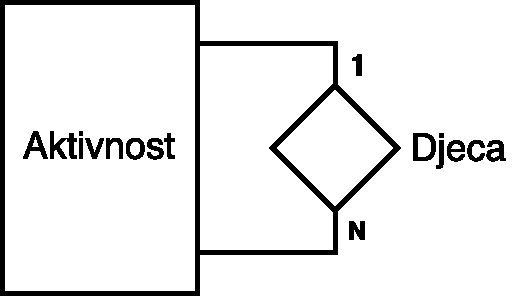
\includegraphics[scale=0.5]{img/refleksivna-aktivnost.pdf}
\caption{Refleksivna aktivnost}
\label{fig:refleksivna-aktivnost}
\end{figure}

Sa ovom refleksivnom vezom tipovi aktivnosti i predmeti mogli bi se premjestiti u entitet 'Aktivnost' te tamo biti definirani kao roditelji postojećih aktivnosti. Hijerarhija bi mogla izgledati ovako:

\begin{figure}[H]
\centering
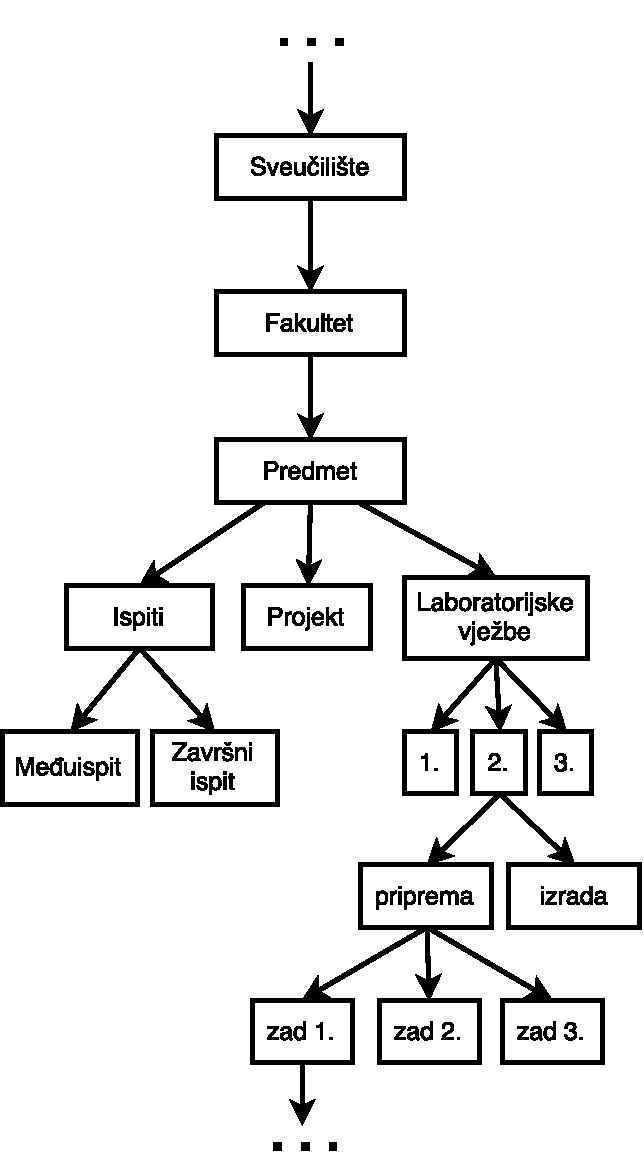
\includegraphics[scale=0.6]{img/stablo-aktivnosti.pdf}
\caption{Stablo aktivnosti}
\label{fig:stablo-aktivnosti}
\end{figure}

Na ovaj način uvijek bi se evidenirale najdublje aktivnosti, a moguće bi bilo prikazivati utrošeno vrijeme zasebno po svakoj dubini stabla, bez obzira na organizaciju ili količinu aktivnosti.
\end{enumerate}

\chapter{Zaključak}
Na osnovu zahtjeva zadatka završnog rada izrađen je ER model baze podataka koji obuhvaća raspon podataka koje je potrebno pohraniti u bazi podataka radi evidencije utrošenog vremena studenata. Zatim je ER model preveden u relacijski model iz kojeg je stvorena baza podataka u Visual Studio okruženju. Na osnovu stvarne baze podataka uz pomoć Entity Framework mogućnosti - obrnutog inženjerstva - stvoren je model koji odgovara stvarnoj bazi podataka.

Web aplikacije razvijena je u više koraka. Prvo je određena podjela web aplikacije: sustav za prijavljivanje, pretplaćivanje korisnika, evidencija utrošenog vremena i pregled statistike. Nakon toga napravljeni su kosturi upravljača i pregleda, te je definirano zajedničko korisničko sučelje web aplikacije (glavni izbornik).

Zatim su napravljeni testni dijelove web aplikacije gdje su se uz pomoć osnovnih formi mogle unositi evidencije i pregledavati statistika kako bi se provjerila ispravnost strukture baze podataka i algoritma koji izračunava statistiku. 

Nakon svih priprema, web aplikacija napravljena je dio po dio, uz pomoć odgovarajući JavaScript biblioteka:
Prvo je napravljen pregled statistike sa Chart.js grafovima, zatim je dodano evidentiranje vremena preko kalendara uz pomoć FullCalendar-a, nakon čega je dodano pretplaćivanje na predmete putem Bootstrap Dual Listbox-a. Na kraju je dodatno izrađen sustav za prijavu i registraciju korisnika i poboljšan stil aplikacije.

\bibliographystyle{fer}
\bibliography{literatura}

\appendix
\chapter{Algoritam računanja statistike}
\lstset{style=csharp, numbers=left}
\lstinputlisting{code/statistika.cs}

\begin{sazetak}

Izrada web aplikacije podrazumijeva izradu odgovarajuće baze podataka. Baza podataka predočuje se pomoću ER konceptualnog modela. Na osnovi ER modela neposredno se izvodi relacijski model baze podataka. Iz relacijskog modela stvara se stvarna baza podataka, koja se zatim obrnutim inženjerstvom pretvara u model koji koristi Entity Framework. Web aplikacija koristi MVC arhitekturu gdje se odvajaju domene modela, upravljačke logike, i korisničkog sučelja. Uz pomoć Ajax-a ostvaruje se asinkrona komunikacija klijenta i poslužitelja. JavaScript biblioteke omogućuju dodatne funkcionalnosti web aplikacije (grafovi i kalendar).

\kljucnerijeci{evidencija vremena, ER model baze podataka, relacijska baza podataka, model-upravljač-pogled, asinkrona web aplikacija}
\end{sazetak}

\engtitle{Database and Web application for study time management}
\begin{abstract}
Creation of a web application assumes the creation of a corresponding database. The database is represented by a conceptual ER model. A relational database model is produced directly from the ER model. The relational model is used to create a real database, from which a corresponding Entity Framework model is generated using reverse engineering. The Web application uses the MVC architecture, which separates the domains of the model, the controller logic, and the user interface. Using Ajax, the client and the server can communicate asynchronously. JavaScript libraries enhance the capabilites of the web application (graphs and the calendar). 

\keywords{time recording, ER database model, relational database, model-view-controller, asynchronous web application}
\end{abstract}

\end{document}
